\begin{itemize}
	\item many many plots (Contour Plots of Surface Currents at 100 GHz and 1 THz (maybe E-Field as well ?),
	Radiation Impedance)
	\item talk about results and expected effects of NiCr Arms 
	\item target resistances and axpectations
\end{itemize}

\begin{figure}[h]
    \centering
    \hfill
    \begin{subfigure}[b]{1\textwidth}
        \centering
        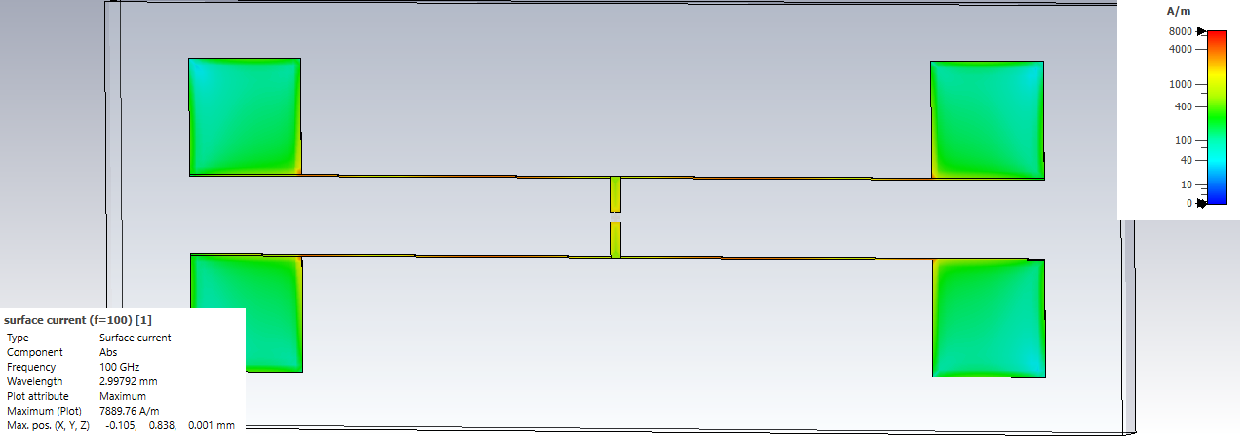
\includegraphics[width=\textwidth]{figures/contour_plots/Contour_ref_0.1THz_SC.pdf}
        \caption{}
        \label{contour_ref_100GHz}
    \end{subfigure}
    \hfill
    \begin{subfigure}[b]{1\textwidth}
        \centering
        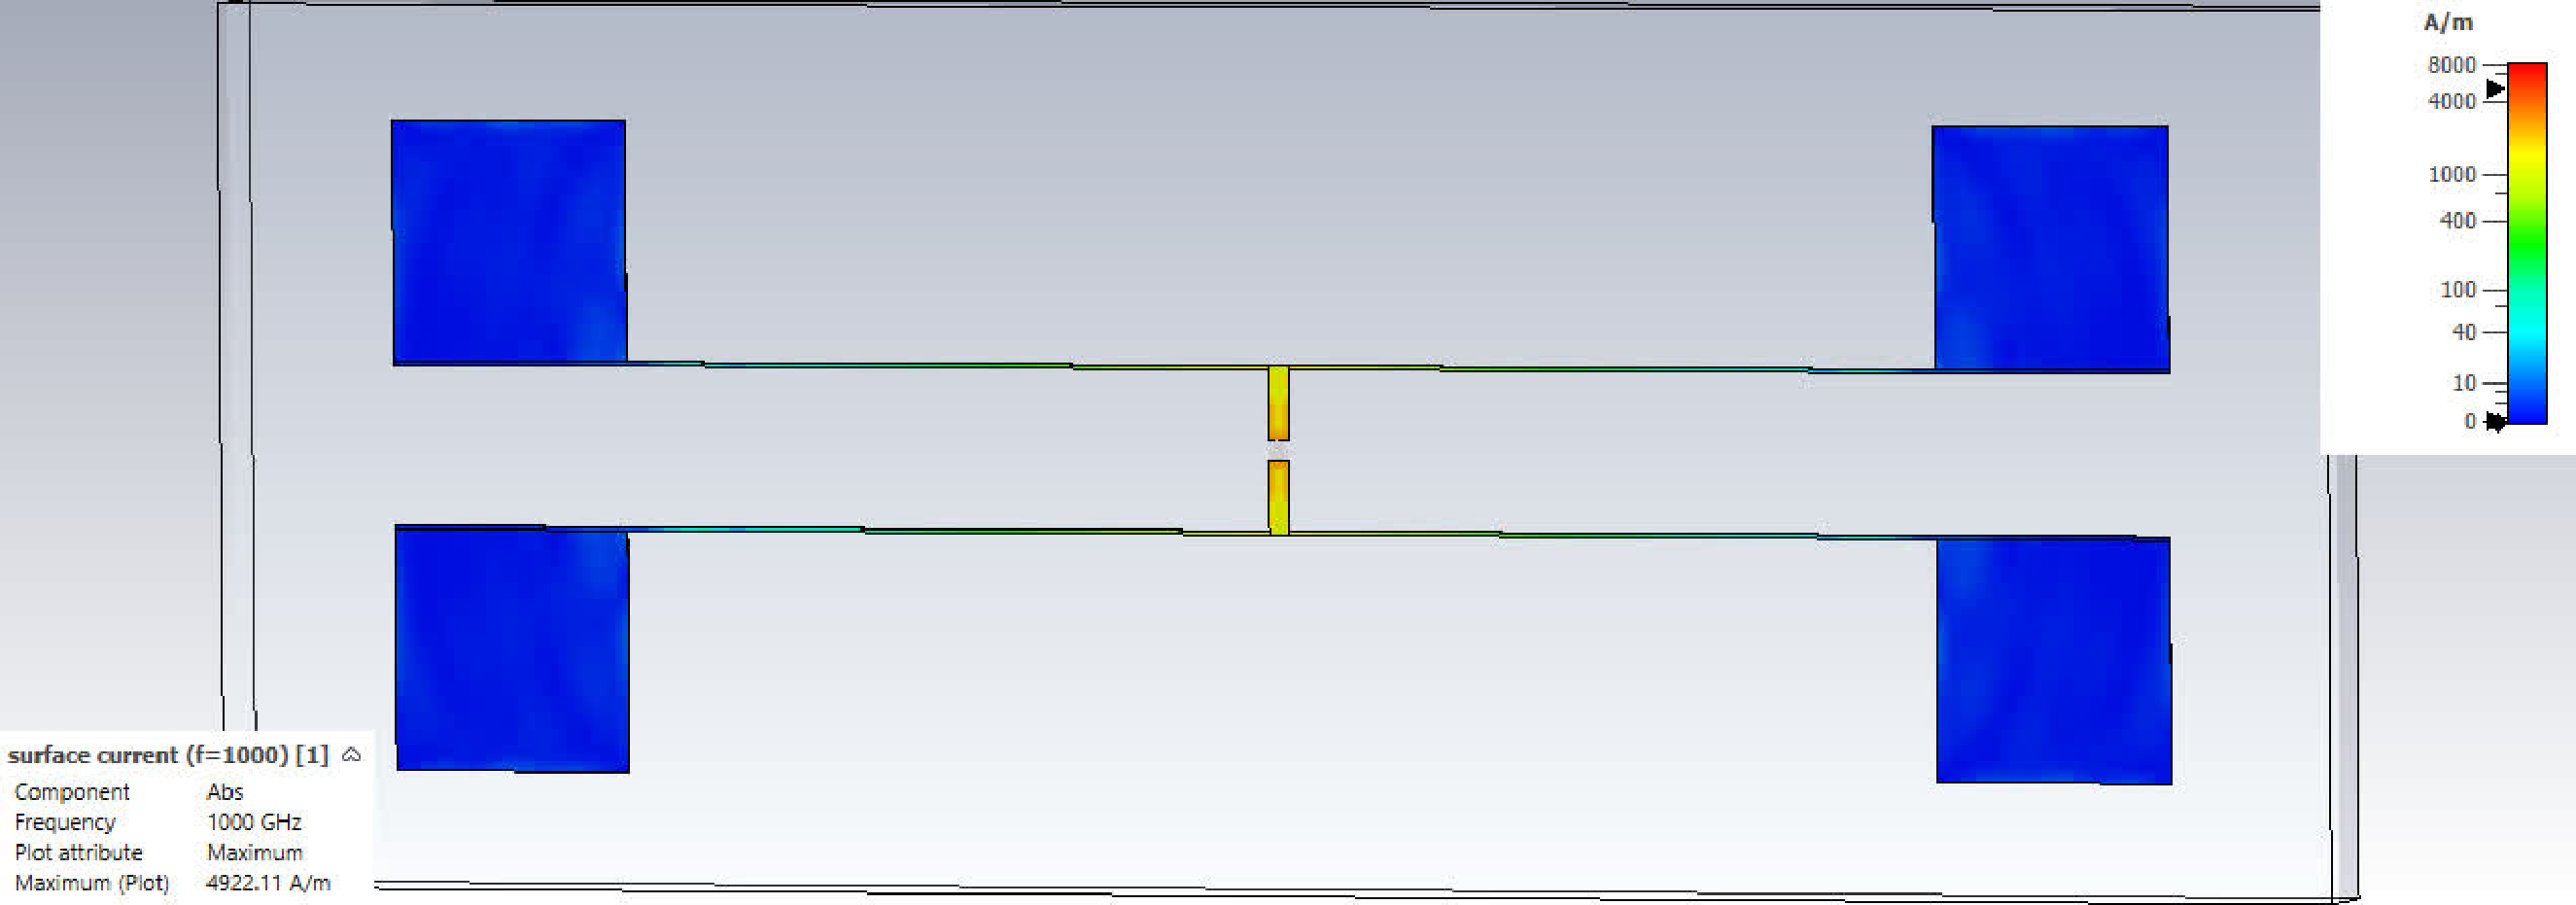
\includegraphics[width=\textwidth]{figures/contour_plots/Contour_ref_1THz_SC.pdf}
        \caption{}
        \label{contour_ref_1THz}
    \end{subfigure}
    \caption{Different PCAs and their general electrode structures are illustrated. Each antenna is designed with rectangular pads for probing. (a) Dimensions of H-Dipole electrodes. (b) Dimensions of bow-tie electrodes. (c) Dimensions of slotline antenna.}
    \label{electrodes_main}
\end{figure}


